% id: 10-17
% book: 100발100중 3-2 중간 · 01 3-2 중간(삼각비·삼각비의 활용·원과 직선·원주각·부록)
% section: 기출 Best
% figure: crop:fig-10-17.png
% answer: ⑤
% answer_source: 답지(빠른정답)
% variant_level: 0 (원본 전사)
% 이 파일은 build.mjs 가 items.json 에서 만든다. 고칠 때는 items.json 을 고친다.
\smash{\raisebox{1.5mm}{\dmkichul{100발100중 3-2 중간 10쪽 17번}}}
$\sin x=0.4848$, $\tan y=0.5774$일 때, 다음 삼각비의 표를 이용하여 $x+y$의 크기를 구하면?
\par\smallskip\begin{center}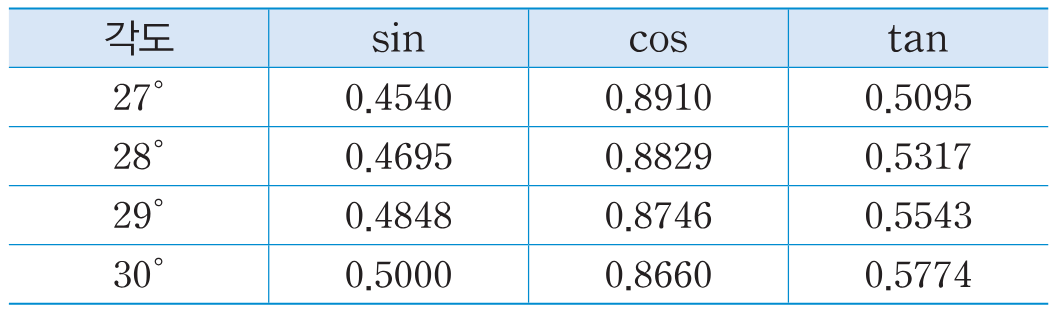
\includegraphics[width=253.4pt]{figures/fig-10-17.png}\end{center}
\begin{choices32}{$55^\circ$}{$56^\circ$}{$57^\circ$}{$58^\circ$}{$59^\circ$}\end{choices32}
